\chapter{Network Compilation}
\label{chap:net_compile}

\section{Layer Decomposition}
\label{chap:net_compile:layer_decomposition}

Given that chip area may be restricted, a hero instance may have
insufficient on-chip storage available to hold ifmap and ofmap memory on chip
during layer processing. To minimize excessive reloads from DRAM we need a way to decompose a
larger layer into sublayers that can fit in the accelerator's on-chip memory.
Decomposition can occur due to either large ifmap or large ofmaps or in some cases
both. In this work it's assumed that decomposition occurs accross channel and
filter axis for input and output feature maps. Decomposition can occur by
decomposing large fmaps along the width and height dimentions however that
complicates the process of aggregating sub layers. This is due to the potential overlaps
of kernel windows accross decomposition boundaries. This issue arises
specifically with (3, 3) kernels under direct mode in HERO. In layers with (1,
1) kernel sizes no overlaps accross decomposition boundaries can occur due to
the small kernel size. 

Depending on the cause of layer decomposition, the dimensionality of either the
input or output featuremaps may change. Beginning with the case of decomposition due
to large ifmap tensors, \autoref{fig:ifmap_decomposition} shows how an ifmap
of size (4, 4) with 4 channels is decomposed into two separate ifmap tensors
each with 2 channels. Each sub layer consists of half the ifmap tensor. Sub
layers are processed sequentially. When
processing the second sub layer a bias is assumed to be loaded in which contains
the partial sums from the first sub layer's output. Once the second sub layer's
output is computed the final ofmap for the filter being processed becomes
available. An illustration of how ifmap decomposition affects weight tiling is
available in \autoref{fig:ifmap_decomposition:weight_tiling}. When decomposing a
large featuremap along the channel axis, the weight tensor has to also be
decomposed. Using the tiling representation of weight tensors, ifmap based
decomposition halves the size of tiles being processed by the architecture. 


\begin{figure}[ht]
    \centering
    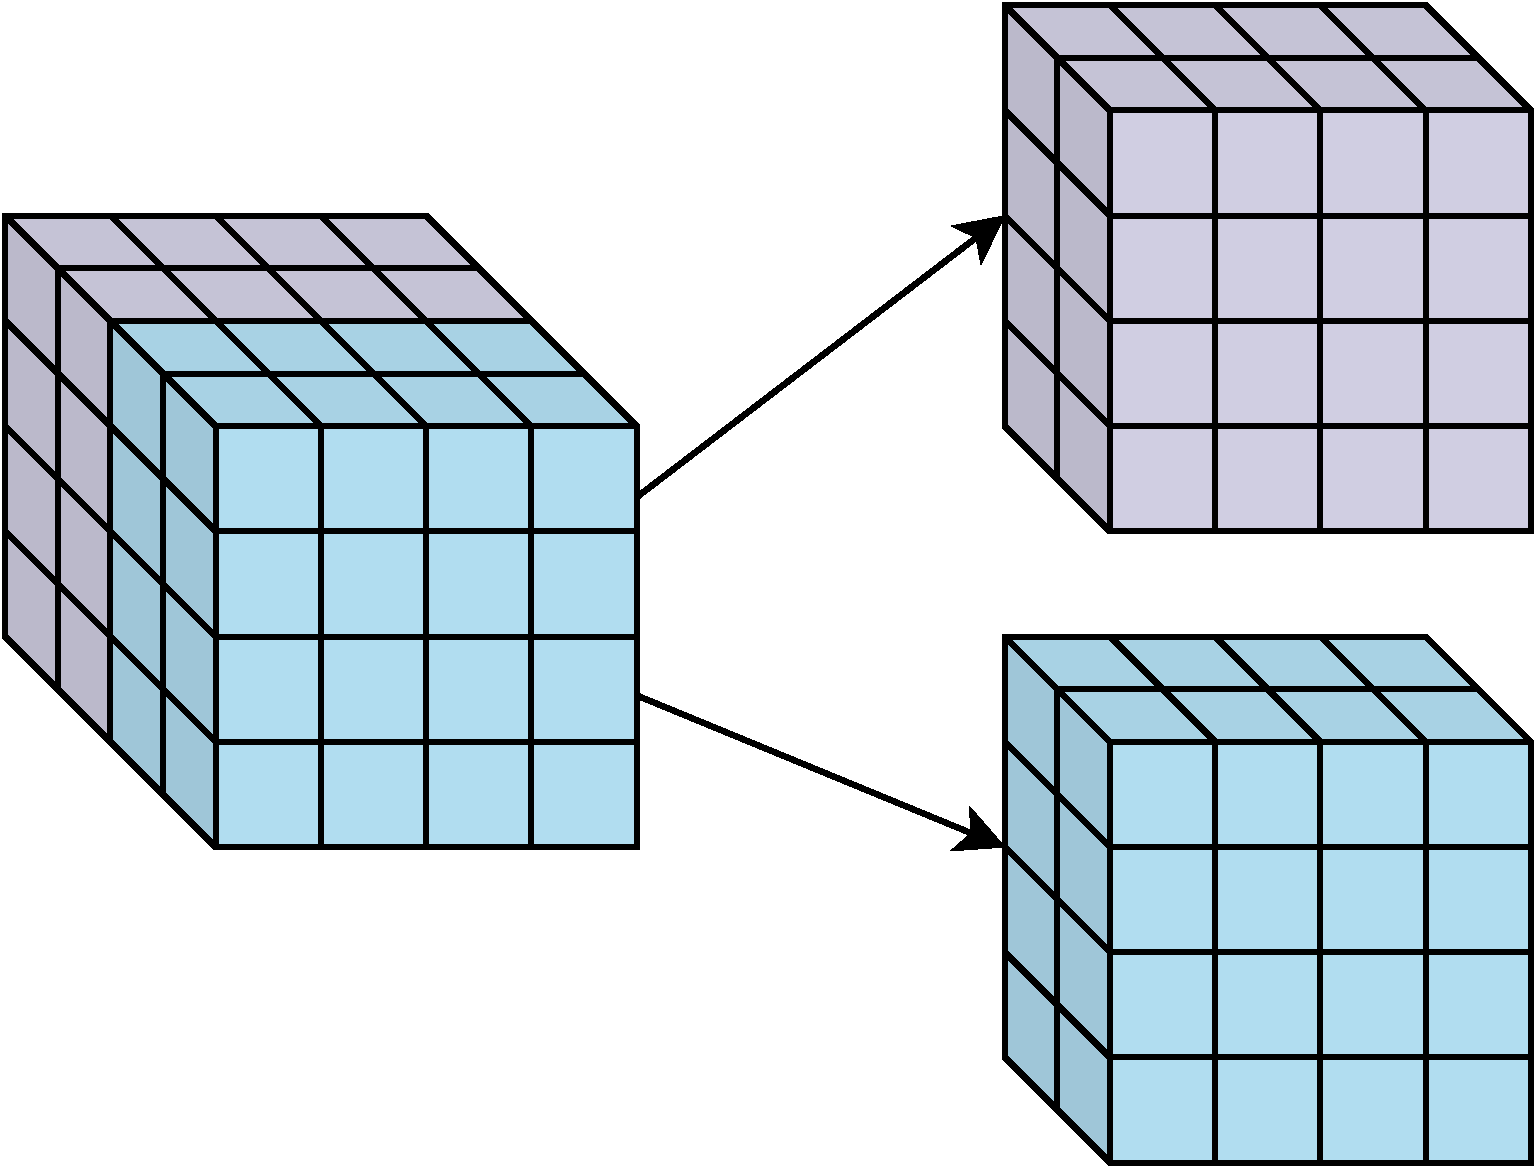
\includegraphics[scale=0.25]{fig/ifmap_decomposition.pdf}
    \caption{Illustration of layer decomposition's effect on Ifmap tensors}
    \label{fig:ifmap_decomposition}
\end{figure}


\begin{figure}[ht]
    \centering
    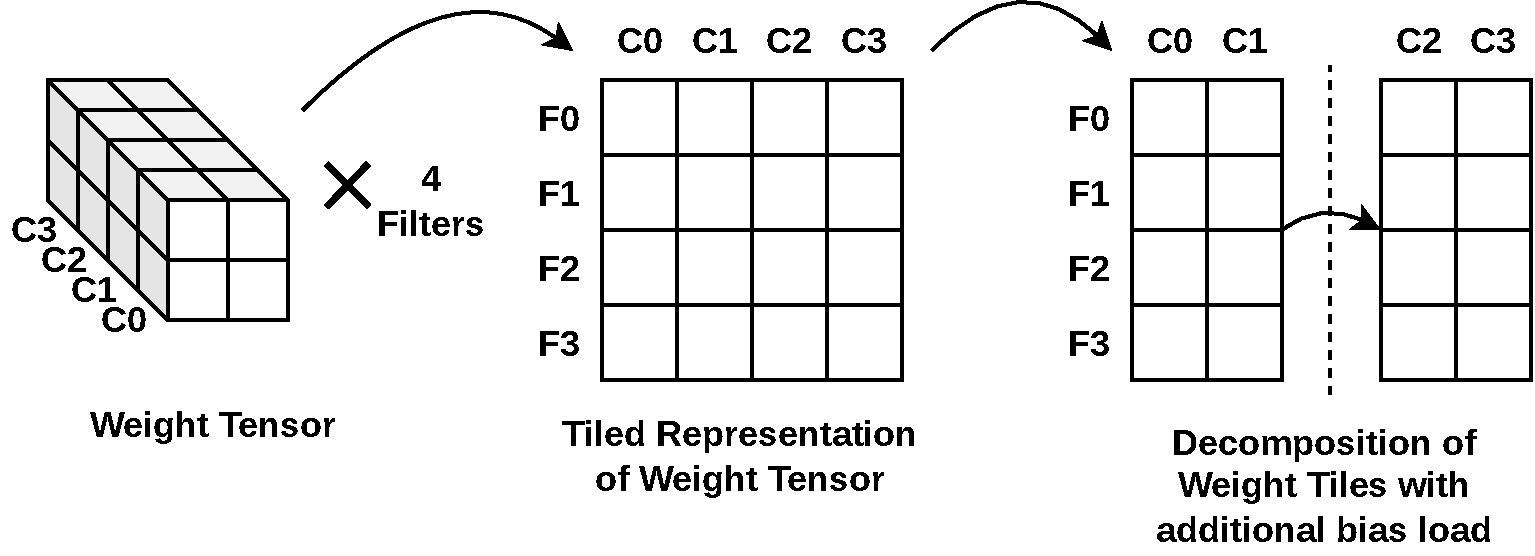
\includegraphics[scale=0.4]{fig/ifmap_decomposition_tiling_repr.pdf}
    \caption{Illustration of layer decomposition's effect on weight tiling}
    \label{fig:ifmap_decomposition:weight_tiling}
\end{figure}

Decomposition due to large ofmaps follows the same logic as in the ifmap case.
An illustration of ofmap based decompsotion is available in
\autoref{fig:ofmap_decomposition:weight_tiling}. If on-chip memory is
insufficient for storing partial sums of large ofmaps from different the layer will be
decomposed into sub layers that will process only a portion of the available
filters in the layers. Ofmap based layer decomposition is also used when
processing depthwise convolution layers given that they are not supported
directly by HERO.  

\begin{figure}[ht]
    \centering
    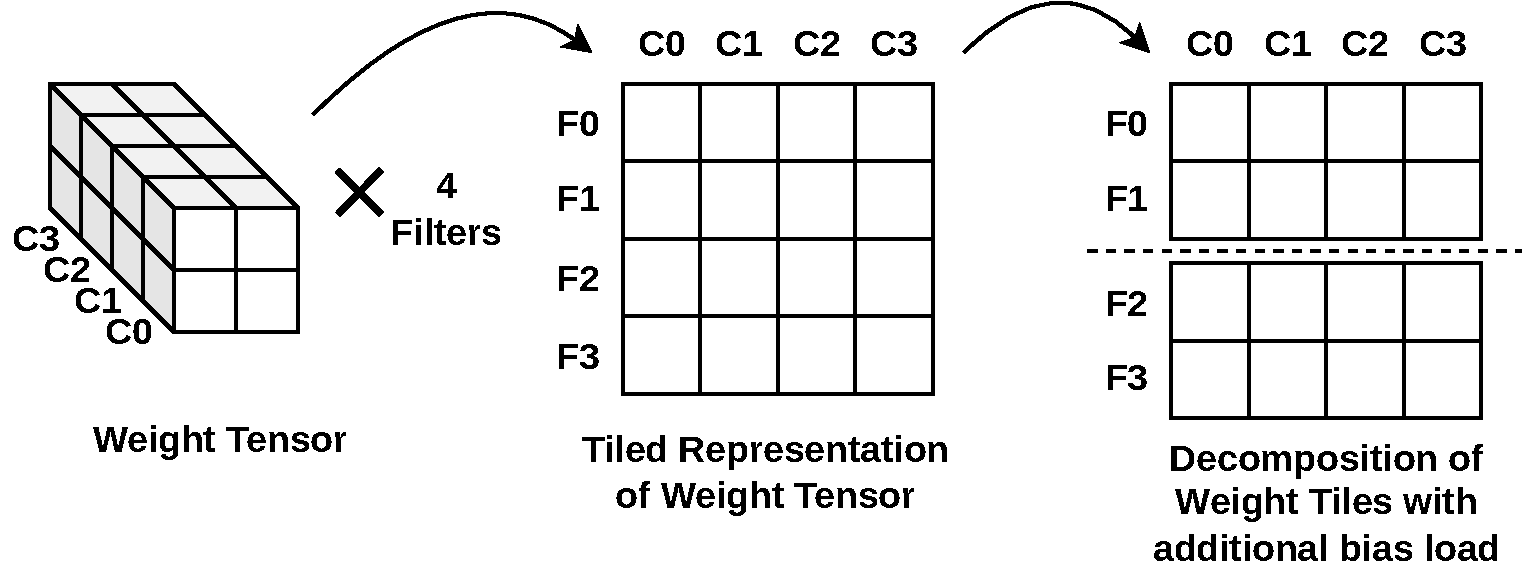
\includegraphics[scale=0.4]{fig/ofmap_decomposition_tiling_repr.pdf}
    \caption{Illustration of layer decomposition's effect on weight tiling}
    \label{fig:ofmap_decomposition:weight_tiling}
\end{figure}

Decomposition primarily affects PE utilization since it may limit available
concurrency when processing channels and filters. In some cases it may cause a
significant reduction of PE utilization. In cases of low utilization due to
layer decomposition other forms of concurrency may need to be supported beyond
the filter/ channel/ kernel concurrency chosen by HERO. An exploration of other
forms of concurrency is left as part of future work. 

\section{Layer Scheduling}
\label{chap:net_compile:layer_scheduling}

On-chip storage requriements for ifmaps and ofmaps are influenced by the
ordering of tiles in the tiling representation of weights discussed in
\autoref{chap:dda}. The order of processing weight tiles is equivelent to the
ordering of the F, and C loops in the loop based representation of the
convolution operation discussed in \autoref{chap:dda}. Processing tiles in F, C
order (ASAP) results in retiring output featuremaps as soon as possible while retaining
input featuremaps for as long as possible. Conversly, processing tiles in C, F
order (ALAP) retains output featuremaps for as long as possible while retiring ifmaps
as soon as possible. An illustration of ASAP and ALAP tile schedules in
available in \autoref{fig:tile_scheduling}. 
% In the final template there are 4 template parameters that are customizable
% depending on the target performance/area/energy efficiency requirements of the
% acclerator. The first and the second are the unroll factors for filters
% ($F_{unroll}$) and channels ($C_{unroll}$). The third is the set of directly
% supported kernels. Finally the fourth is the spatial axis mapping of the kernel
% loops ($K_{axis}$). Each of these parameters has an effect on on-chip storage
% required for the different memories accessed.

\begin{figure}
    \centering
    \subfigure[]{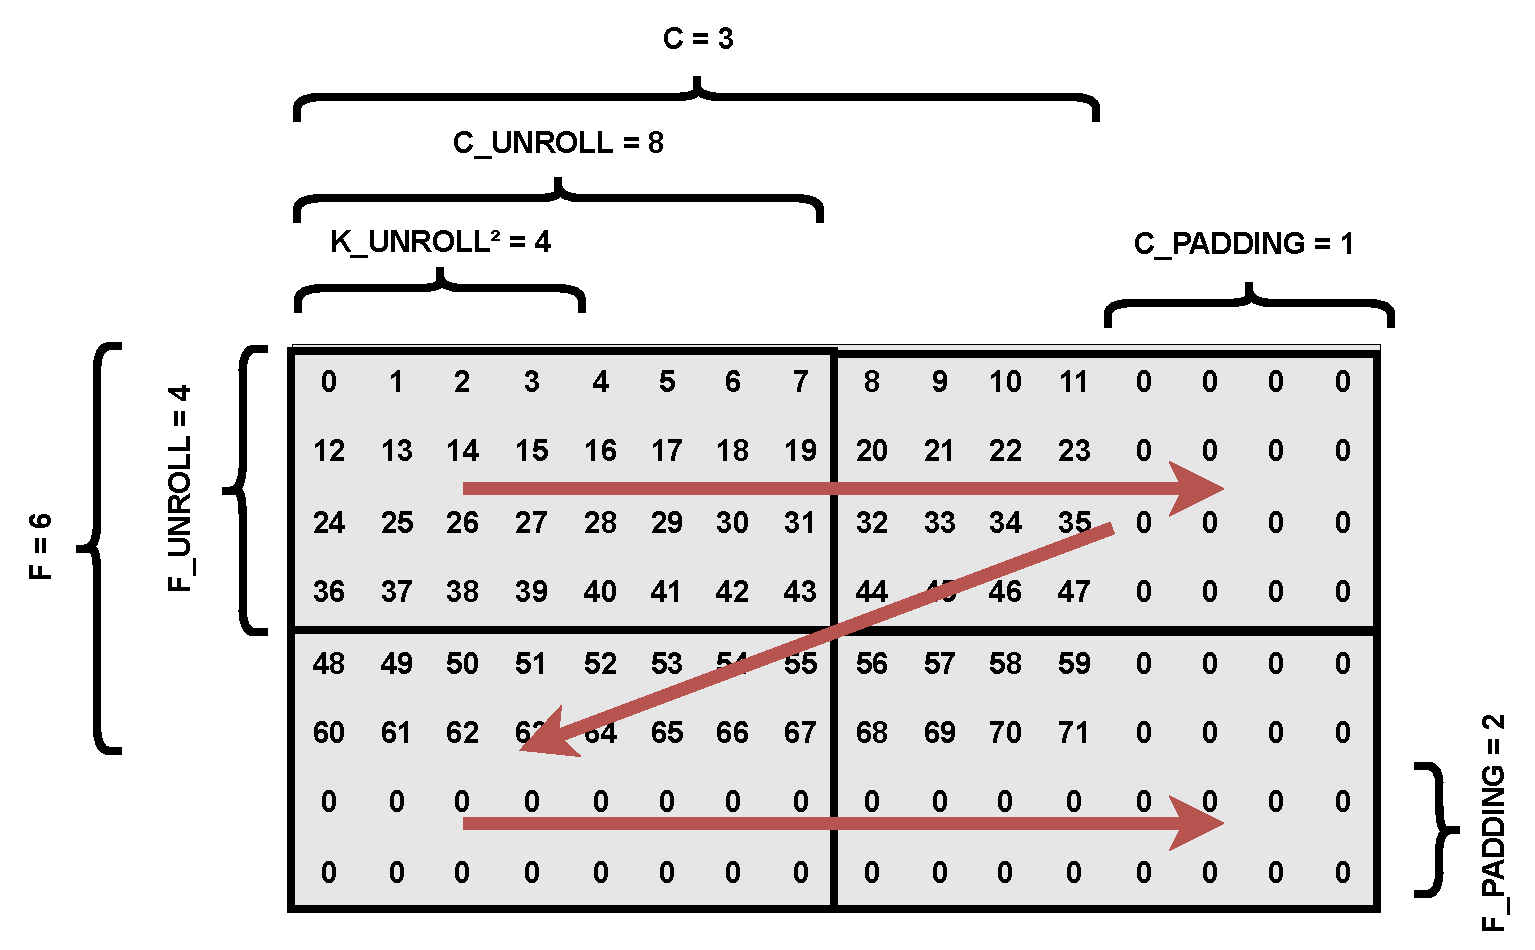
\includegraphics[width=1\textwidth]{fig/asap_tiling.pdf}}
    \hspace{0.1cm} 
    \subfigure[]{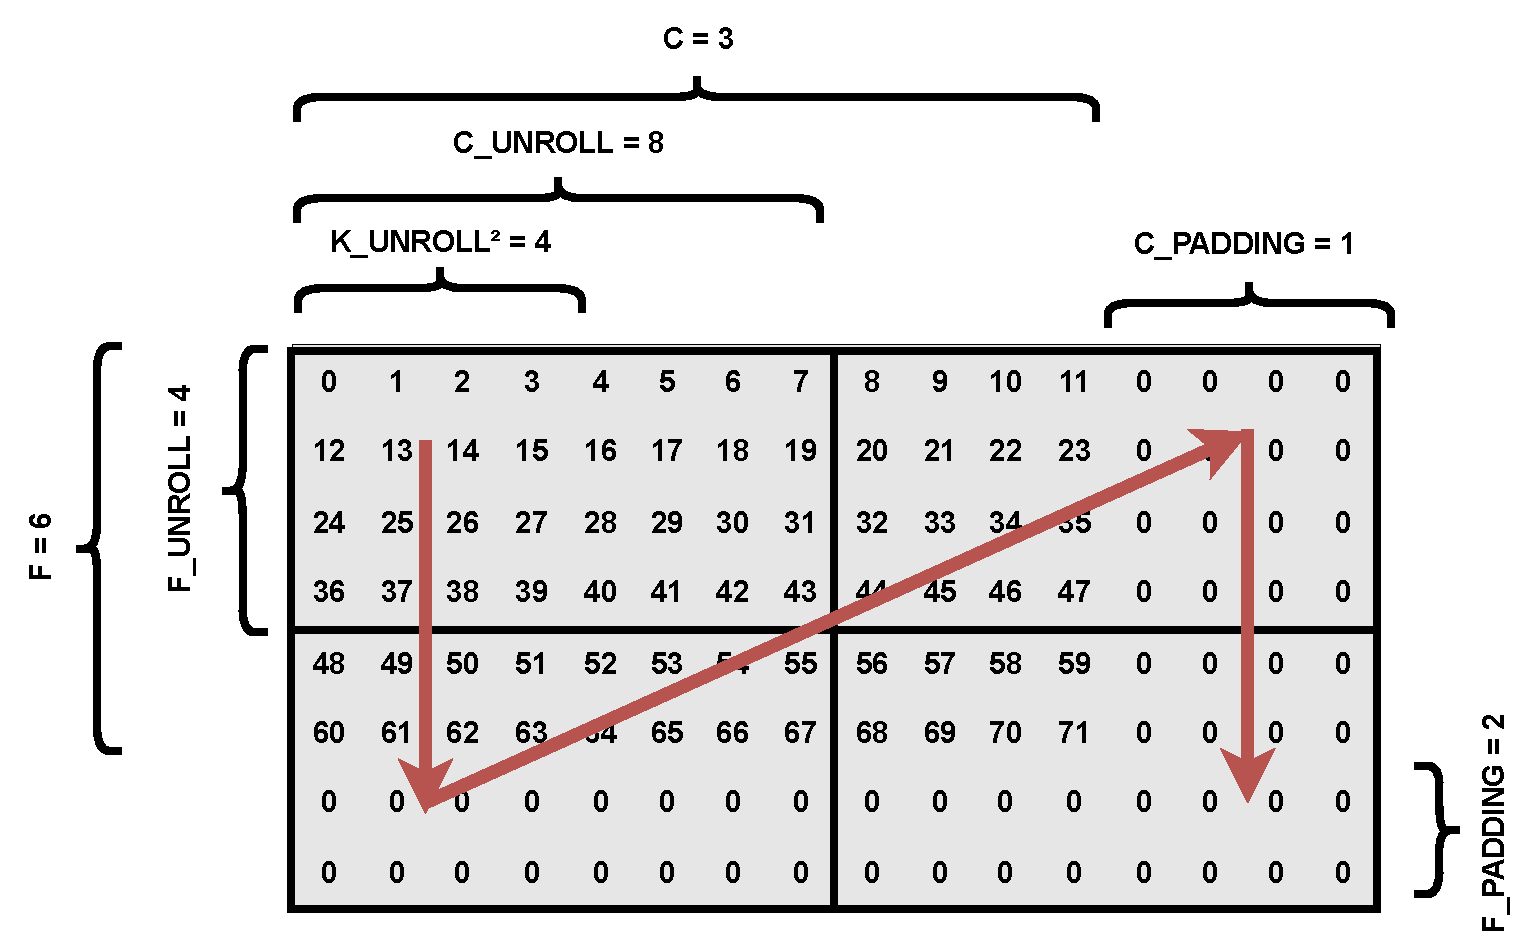
\includegraphics[width=1\textwidth]{fig/alap_tiling.pdf}}
    \caption{Illustration of different tiling schedules (a) ASAP scheduling (F, C)  (b) ALAP scheduling (C, F)}
    \label{fig:tile_scheduling}
\end{figure}

An illustration of this architectural tradeoff is present
in \autoref{fig:Fmap_scaling}.c. Note that depending on the tile scheduling
chosen, different HERO template parameters affect the scaling of different
on-chip memories. For example, under ASAP, input featuremap memory requriements
remain unchanged with any template parameters, however, ofmap memory scales
with the architecture's filter unroll factor. Under ALAP ofmap memory remains
unaffected by any of HERO's template paramaters, however, ifmap memory scales
with the architecture's channel unroll factor. An illustration of how both
memories scale with tempalate paramaters is given in
\autoref{fig:Fmap_scaling}.a \& \autoref{fig:Fmap_scaling}.b. 

\begin{figure}
    \centering
    \subfigure[]{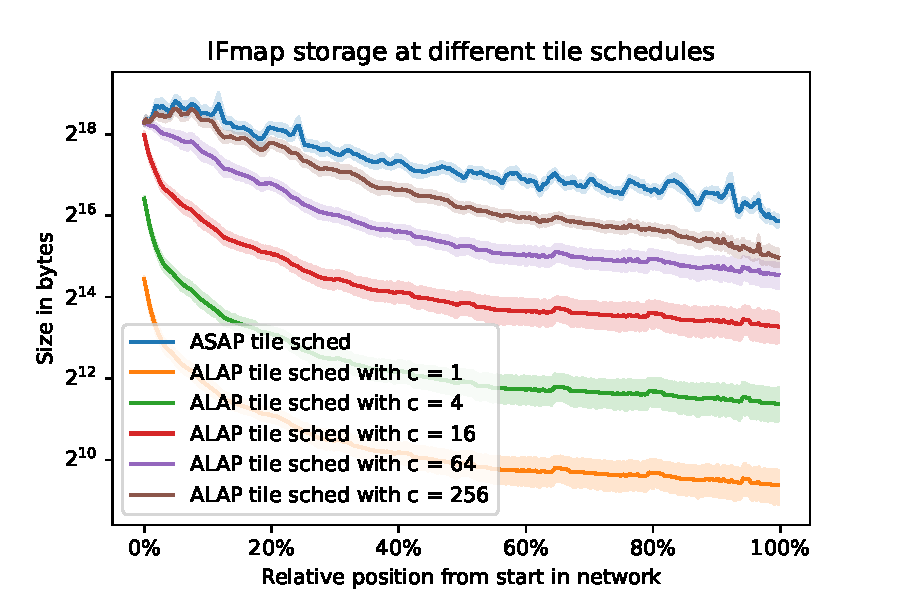
\includegraphics[width=0.45\textwidth]{Plots/ifmap_Storage.pdf}}
    \hspace{0.1cm} 
    \subfigure[]{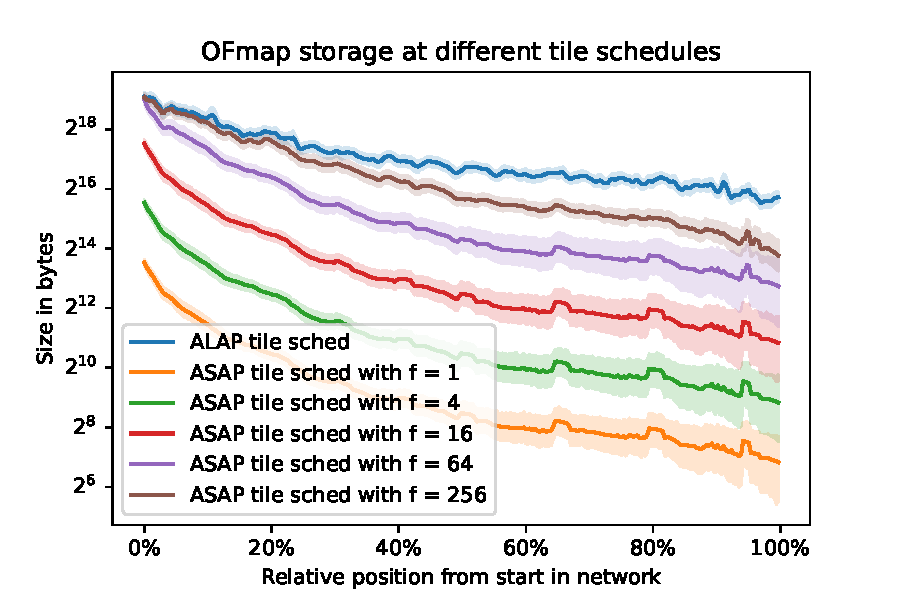
\includegraphics[width=0.45\textwidth]{Plots/PSUM_Storage.pdf}}
    \subfigure[]{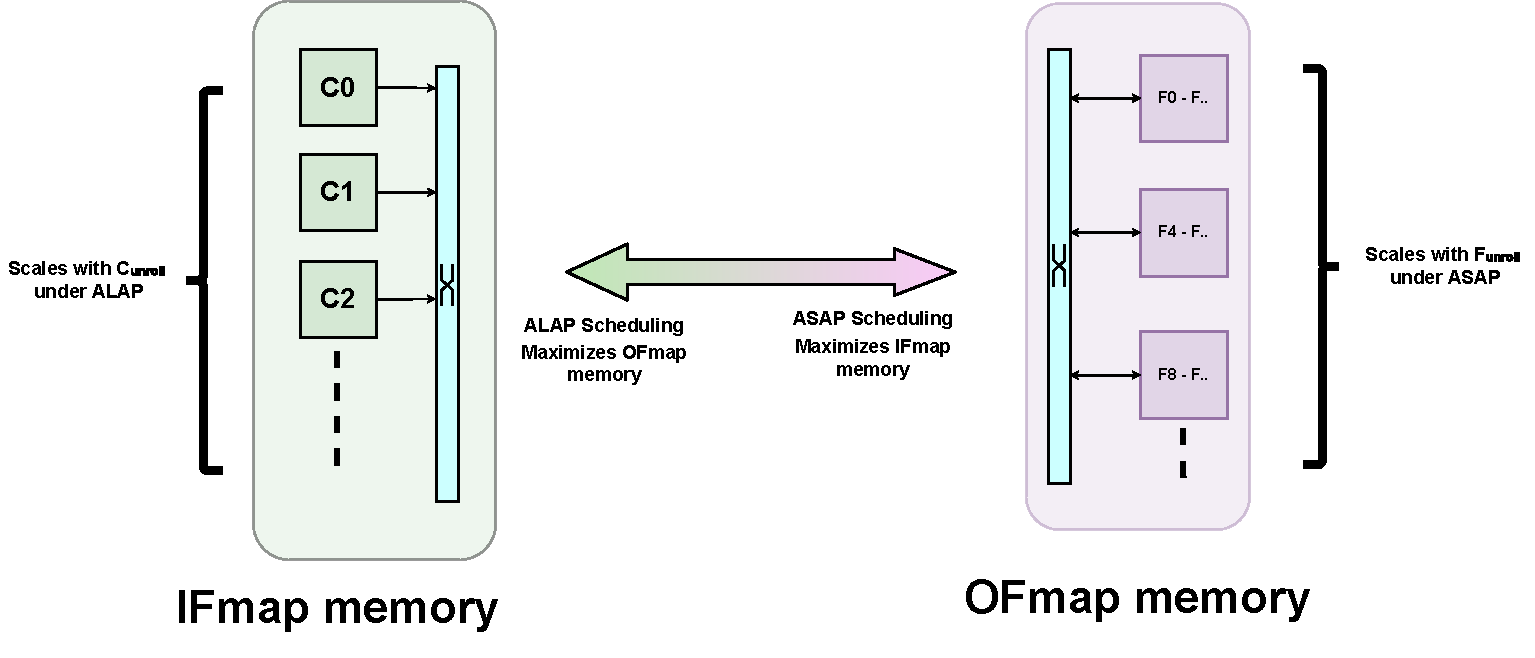
\includegraphics[width=1\textwidth]{fig/psum_ifmap_mem_scaling.pdf}}
    \caption{Illustration of storage tradeoff between OFmaps and IFmaps depending on tile scheduling (loop ordering) and accelerator template parameters (loop unroll factors) (a) IFmap storage (b) OFmap storage (c) archictural illustration}
    \label{fig:Fmap_scaling}
\end{figure}

In this work ASAP scheduling is always assumed given the relatively poor scaling
of ofmap memory with architecture template paramaters. This poor scaling is due
to the necessity of storing ofmap elements using higher precision values to
prevent numeric overflow. Note that in allowing different tile schedules may
sometimes negate the need for layer decomposition. The interaction between layer
decomposition and layer scheduling is left as part of future work.  

% While a weight stationary offers limited flexibility with regards to loop
% reoredering it does offer some degree of flexibiltiy with regards to ordering
% filter loops and channel loops. F, C loop ordering affects required on-chip
% storage for IFmaps and OFmaps.
% Under Direct mode and Gemm mode with balanced lowering, IFmap sizes
% do not exceed $2^{19.25}$ bytes (assuming 8 bit precision) for 95\% of all
% convolution layers in CIGAR's library. An estimation of the
% on-chip area required to store IFmaps using the model presented in
% \cite{area_model} yields a total on-chip area per sram bit stored equal to 0.013
% $um^2$ which translates to $0.064 mm^2$ on-chip area dedicated to sram buffers
% for storing entire input feature maps for a layer at 14nm technology.
% This area/storage does not scale with increased/decreased filter unroll factor,
% channel unroll factor or max directly supported kernel size. On-Chip area
% dedicated to storing Weights scales with the afformentioned parameters.
% Storage with regards to OFmaps depends on the loop ordering in the chosen
% dataflow. Specifically on-chip OFmap storage depends on whether filter loops and
% channel loops are reordered such that OFmaps are retired as fast as possible
% (ASAP tile scheduling) by iterating through IFmap channels first while
% processing a groups of filter, or as late as possible (ALAP tile scheduling) by
% iterating through filters first while processing a group channels. These two
% orderings for filter loops and channel loops represent different tile schedules
% for processing convolution layers. An illustration of both tile scheduling
% approaches is illustrated in \autoref{fig:tile_scheduling}. In
% \autoref{fig:tile_scheduling} a (1, 1) convolution layer's weights are shown with
% the architecture's unroll factors overlayed on top. The overlay of the
% architecture's unroll factor creates distinct weight tiles where componenets of
% the OFmap are computed. The order of executing these weight tiles depends on the
% chosen tile schedule. ASAP which represents F, C loop ordering and ALAP which
% represents C, F loop ordering. 

% A tradeoff between required IFmap storage and required OFmap storage is apparent
% in \autoref{fig:fmap_size_trends}. Under ASAP scheduling, storage requirements for
% OFmaps scales with $F_{unroll}$ because $F_{unroll}$ represents the maxmimum
% number of filters in flight. Storage requirements for IFmaps is maximized under
% ASAP because all channel data would need to be held on-chip assuming no
% additional reads can be made from DRAM for IFmap channels. Under ALAP
% scheduling, storage requirements for IFmap scale with $C_unroll$ because
% $C_{unroll}$ represents the maximum number of channels in flight. Storage for
% OFmaps is maximized under ALAP. In this thesis it is assumed that chip
% area (and thus on-chip memory) is always sufficient at least one of the
% afformentioned tile schedules without requiring loop blocking and additional
% DRAM accesses for feature maps. An exploration of the effect of loop blocking
% under more restrictive area constraints is relegated to future work. 

\clearpage

\section{Descriptor Program Generation}
\label{chap:sams:acc_scheduling}

We can generate descriptor programs for the SAMs present in
in the final architecture template for HERO discussed in \autoref{chap:dda:hw_dse:final}.
These descriptor programs will be used to perform memory operations necessary
for the convolution operation to take place in the final architectural template.
It's assumed that all on-chip SRAMs present in the HERO architecture are SAMs
capable of being programmed with descriptor based programs.   
Since we have two operational modes based on the findings of
\autoref{chap:dda} (direct and Indirect mode) we will discuss the
descriptor programs required for both of these modes to take place independently of
the other. Note that indirect mode is just a data transformation operation
followed by a (1, 1) convolution operation as discuseed in
\autoref{chap:dda:dataflow_dse:indirect_mode}. Indirect mode data
transformations (lowering/ lifting) are assumed to be performed off chip. Moving
these transformations on-chip is left as part of future work. This leaves us
with effectively two operations we need to generate descriptors for, (1, 1) and (3, 3)
convolutions. For each operation, descriptor based programs need to be generated
to perform the necessary data transfer operations between on-chip memories and
PEs. It's assumed that all on-chip SRAMs in HERO are SAMs capable of being
programmed with descriptor based memories. 
For now it's assumed that there exists two flexible interconnects for routing
control signals between address generators and on-chip SRAMS. One between all
address generators and banks in Ifmap L3 and another between all address
generators and Ofmap banks. These control interconnects are different from the
data interconnects that allow routing of data from banks to arbitrary output
ports connected PEs. An illustration of this interconnect scheme is available in
\autoref{fig:interconnect}

\begin{figure}[ht]
    \centering
    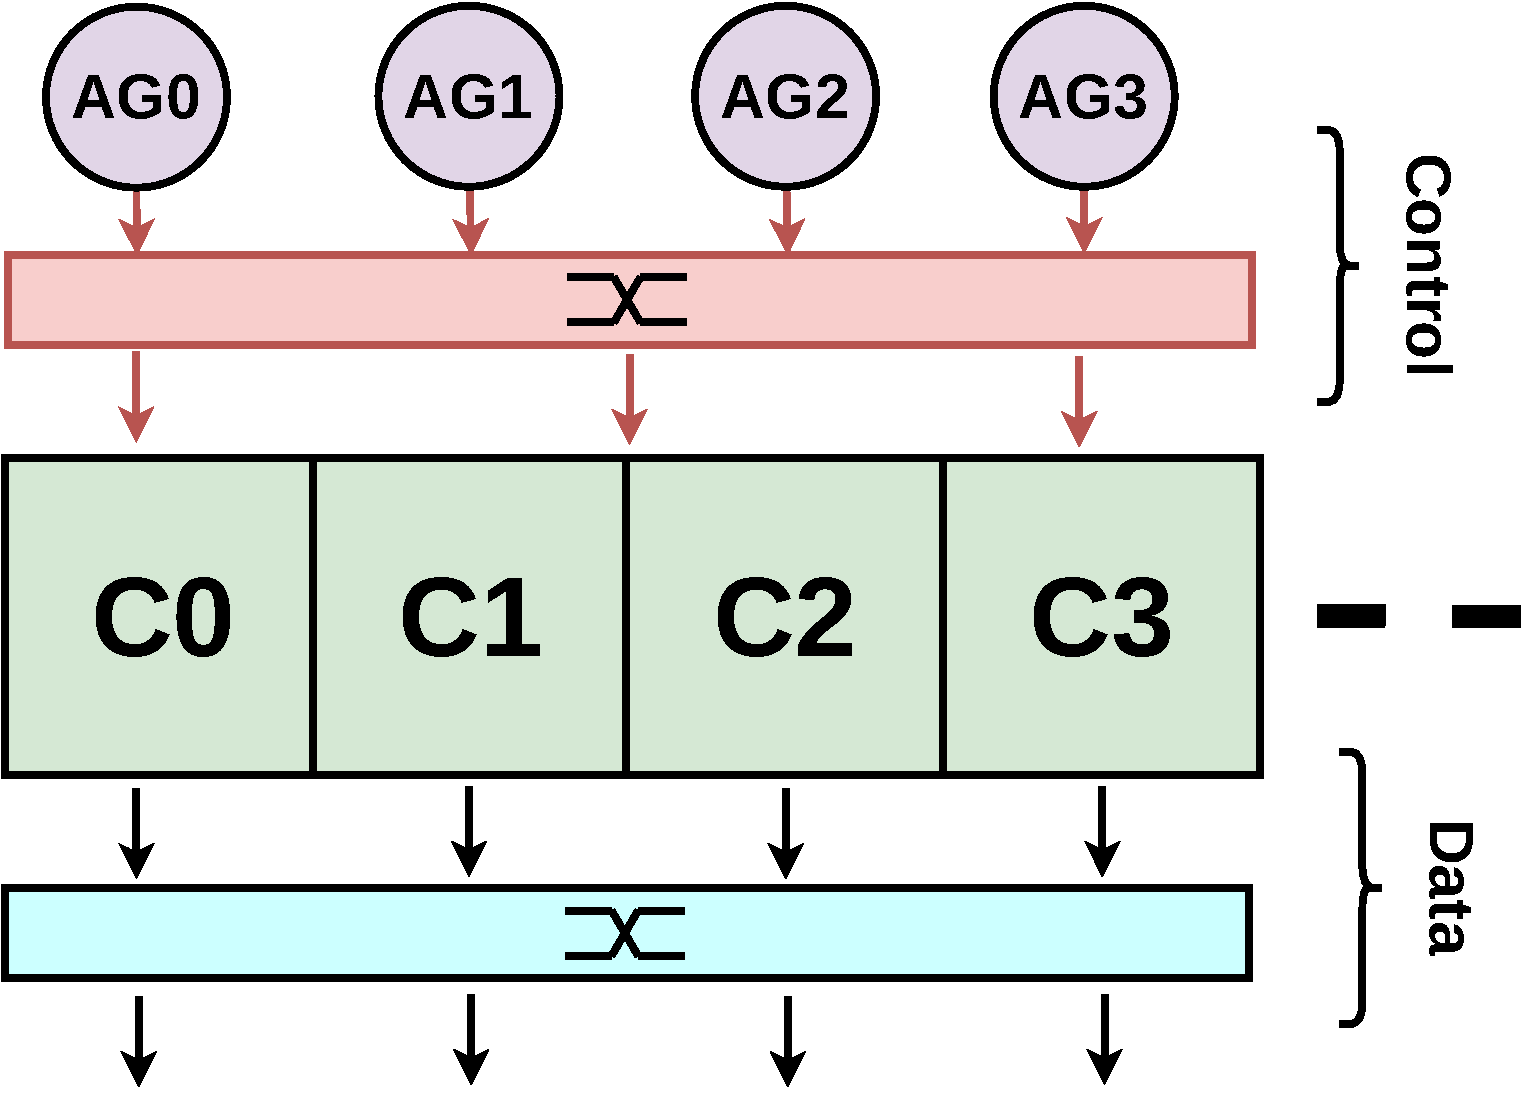
\includegraphics[scale=0.3]{fig/interconnect.pdf}
    \caption{Illustration of interconnects for control and data in on-chip featuremap memories}
    \label{fig:interconnect}
\end{figure}


This flexible interconnect for routing control signals
allows address generators of SAMs to be able to send read/write requests to
different SRAMs connected to the same interconnect which enables arbitrary
access of featuremap banks. This solution is likely not scalable to larger
instances of HERO and will be superceeded by statically scheduled control
interconnects in future work. 
Additionally, all interactions between SAMs and DRAM are left as part of future
work. IFmap and OFmap data is assumed to be read from and written to DRAM before
and after the operation of the SAM programs discussed in thi section. Latencies
and energy penalties associated with DRAM will be considered in
\autoref{chap:results} but the descriptor programs discussed in this chapter are
DRAM agnostic.

\subsection{1x1 convolution programs}
\label{chap:sams:acc_scheduling:1x1}


To illustrate how SAMs can be programmed to perform a (1, 1) convolution we will
use a simplified version of HERO illustrated in \autoref{fig:1x1conv_sched_tiling} and a (1, 1) convolution
layer with 16 channels and 8 filters as a driving example. The simplified
version of HERO assumed that there are a total of 9 processing engines with all 9
mapped to the accelerator horizontal spatial axis which enables creates an
effective an unroll factor of 9 at kernel sizes (1, 1). Based on the tiling
discussion in
\autoref{chap:dda:dataflow_dse:pruning:applying_it:loop_unroll_factors}, the
architecture tiles the weight tensor into 16 tiles (padding included) as
illustrated in \autoref{fig:1x1conv_sched_tiling}.

\begin{figure}[ht]
    \centering
    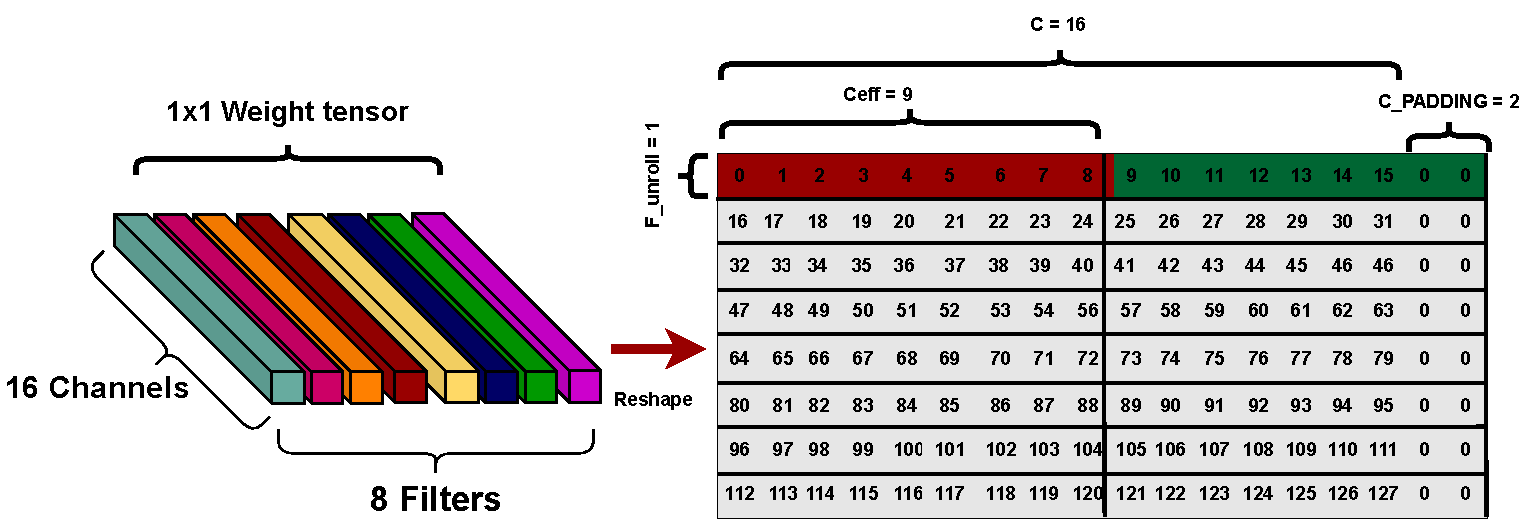
\includegraphics[scale=0.6]{fig/1x1conv_sched_tiling.pdf}
    \caption{Illustration of weight tiling under (1, 1) convolution}
    \label{fig:1x1conv_sched_tiling}
\end{figure}

For each weight in the tiles of \autoref{fig:1x1conv_sched_tiling} the channel
feature map corresponding to that weight has to be streamed into the PE
processing the output of that weight. For example, tile highlighted in red needs
channels C0-C8 streamed into the PEs storing those weights for processing. After
the red tile is processed, the green tile is loaded into the PEs weight buffer
(assuming ASAP scheduling as seen in
\autoref{chap:net_compile:layer_scheduling}). Channels C9-C15 then needs to be
streamed into the PEs holding the weights corresponding to those channels. This
means that channel memories may need to hold multiple channels that are streamed
out depending on the index of the tile being processed. An illustration of how
channel feature maps are stored on the channel SAMs is present in
\autoref{fig:channel_banking}. Note that in cases where channel featuremaps
exceed the size of one bank, layer decomposition spreads the feature map accross
multiple banks. This causes a reduction in available channel concurrency which
leads to low PE utilization. PEs holding 0 valued weights due to padding have no
corresponding channel data so nothing is streamed into them as reflected in the
0 padding of the last channel SAM attached to the 9th PE in
\autoref{fig:channel_banking}. Additionally, they are assumed to just forward
any partial sums/ output feature maps recieved from their input to their output
with no modifications.

\begin{figure}[ht]
    \centering
    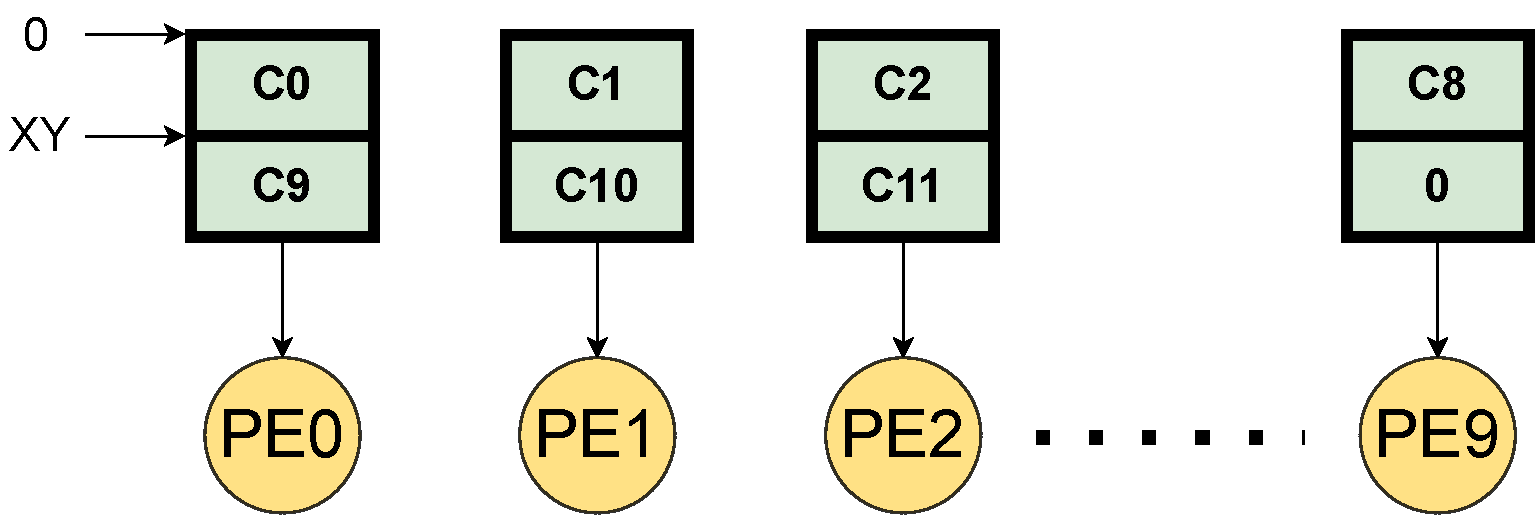
\includegraphics[scale=0.495]{fig/1x1conv_ifmap_banking.pdf}
    \caption{Illustration of channel banking in Ifmap L3 on-chip SRAMs}
    \label{fig:channel_banking}
\end{figure}

Since (1, 1) convolutions involve entire channel feature maps streamed into PEs
with no reuse within a feature map occuring as in the (3, 3) case, the only
memories that need to be programmed are the L3 channel memories and the OFmap
memories. An illustration of the required descriptor programs for the
afformentioned memories is given in \autoref{fig:1x1conv_sched}. In
\autoref{fig:1x1conv_sched} hirarchy layers unused by the computatation 
as well as some PEs have been ommited to for brevity.

\begin{figure}[ht]
    \centering
    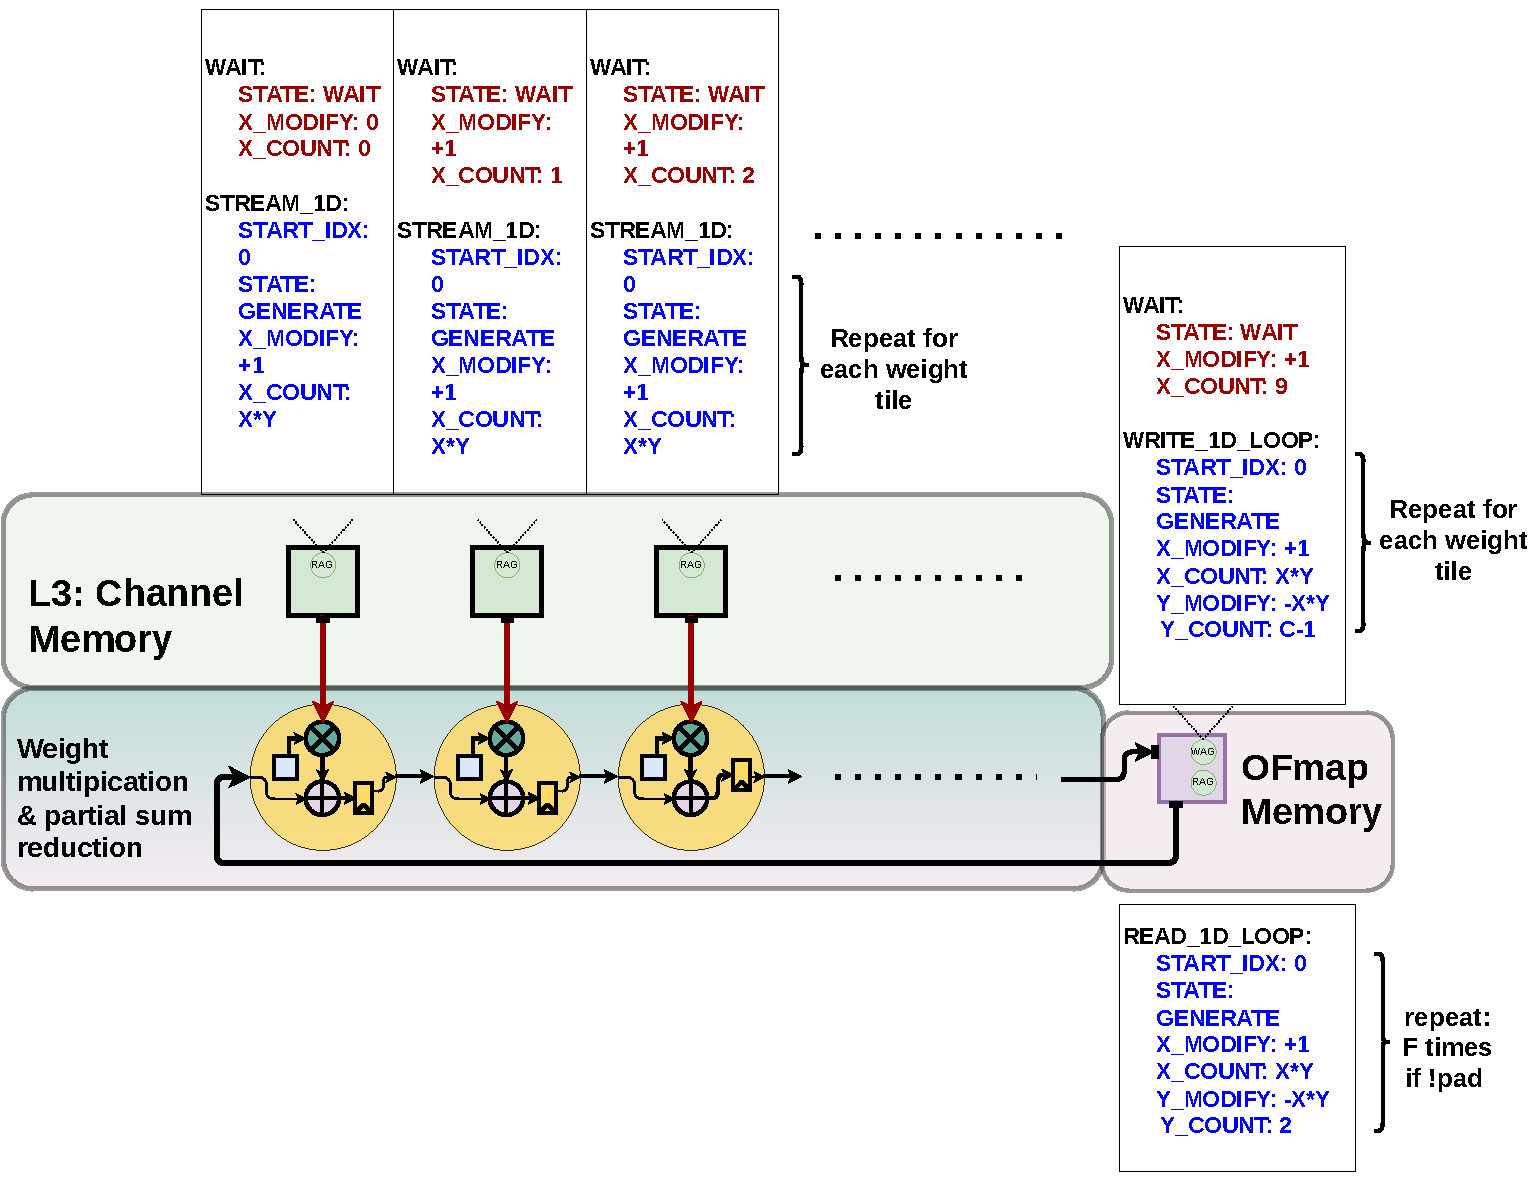
\includegraphics[scale=0.495]{fig/1x1conv_sched.pdf}
    \caption{Illustration of (1, 1) convolution scheduling}
    \label{fig:1x1conv_sched}
\end{figure}

In \autoref{fig:1x1conv_sched} channel memories can be implemented with SAMs.
For each channel SAM there are two descriptors types that appear frequently in
their programs, a wait descriptor and generate descriptor. Channel SAMs need to
perform timed reads due to the systolic delays arising from the systolic
reduction of partial sums into output feature maps. Therefore, an initial wait
instruction due to the systolic delay required by each SAM is inserted at the
begining of their descriptor programs. The delay defined by the wait descriptor
for each SAM depends on the index of the PE that the SAM is connected to. So the
first PE's corresponding SAM has no read delay so the x\_count variable in the
wait descriptor is set to 0. The next PE's channel SAM has a delay of 1 so it's
initial weight descriptor's x\_count is set to 1. After the initial wait
descriptor, each channel SAM needs to stream out a feature map. Depending on the
index of the tile being processed, each SAM streams out a different IFmap. What
distinguishes each IFmap stored on a channel SAM from another is it's start
index. For example, for the first tile highlighted in red, the first PE streams
out the IFmap begining at start index 0 with a generate descriptor. The size of
that IFmap is assumed to by $XY$ where $X$ and $Y$ are the width and height of
the IFmap. The generate descriptor increments the internal address "addr" $XY$
times with "addr" starting at 0. The corresponding generate descriptor that
manipulates the "addr" like that is a generate descriptor with an x\_count of
$XY$ and a start index of 0. When the first PE begins processing the second
tile, it reads out the IFmap stored at index $XY$ or more generally
$MOD(tile_{idx},2).XY$ since each filter has 2 tiles. This generate descriptor
is repeated for each tile in the weight tensor assuming that no padding. If a PE
is storing a 0 valued weight due to padding the generate descriptor is replaced
with a wait descriptor with an x\_count of $XY$. Optimizating descriptors to
reduce code size is left as part of future work.

For the OFmap SAM two address generators are required due to the read modify
write nature of OFmaps. The read port begins reading the layer bias immediately
and streams it into the first PE as part of partial sum reduction. All later
reads from the OFmap SAM are for partial sums that have yet to be accumulated
into OFmaps. The read descriptor required for streaming in bias/ partial sums is
a generate descriptor that streams out the contents of OFmap in a loop. It
achieves this by setting x\_count to $XY$ to stream out partial sums of size
$XY$ and y\_count to 2 which the number of tiles in a filter. To reset the
"addr" index of the read descriptor the y\_modify is set to $-XY$. This generate
descriptor is repeated 8 times where 8 is the number of filters present
processed by the PEs assuming no filter padding. Assuming ASAP tile scheduling,
OFmaps are written to DRAM as soon as they are completed and are not kept on
chip.

The write port waits for $C_{UNROLL}$ number of cycles to write the first
partial sums that will eventually become OFmaps once the filter being processed
concludes. IFmaps of $XY$ size less than 9 (the number of PEs in the horizontal
axis) will cause additional delay cycles to be introduced via wait descriptors
to allow partial sums to propogate through the PEs to reach the OFmap.
 The descriptor required for
the write address generator are similair to the the read ones with the exception
of an additional wait descriptor that gives the first partial sum/ Ofmap time to
propogate through the systolic reduction. The delay required by the wait
descriptor is equal to the number of PEs present in the horizontal axis. After
the wait descriptor comes a generate descriptor that writes the partial sum
output/ OFmap output into the OFmap SAM in a loop. The write generate
descriptor is repeated 8 times as well assuming no padding similair to
the read generate descriptor.

\subsection{3x3 convolution programs}
\label{chap:sams:acc_scheduling:3x3}

Since (3, 3) convolution operations involve the ifmap L2 vertical reuse memory,
data transfer operations between L3 an L2 have to be performed by the descriptor
based programs in memories of both layers. Thankfully, the programs for L3
memories are similair to the (1, 1) convoltuion case where each memory streams a
series of ifmap channels after a systolic delay. The main difference between (3, 3)
and (1, 1) L3 programs is is the existence of an initial setup phase where the
first two lines of a featuremap are transferred into the L2 followed by a delay
that allows partial sums to propogate down to the set of PEs each L3 featuremap
bank is connected to. Once this setup phase concludes the rest of the
featuremap is streamed out in the run phase. These two phases are repeated for every
weight tile in the layer. The L2 memory acts as a series of programmable fifos
that emit featuremaps after a delay determined by the width of the featuremap.
They also have an additional setup phase that enables them to recieve the first
two lines from L3 channel memories and then wait until partial sums begin
propogating to the OFmap memory. 
An illustration of this behavior is given in \autoref{fig:mlti_ag_ops}.b. 


\begin{figure}[ht]
    \centering
    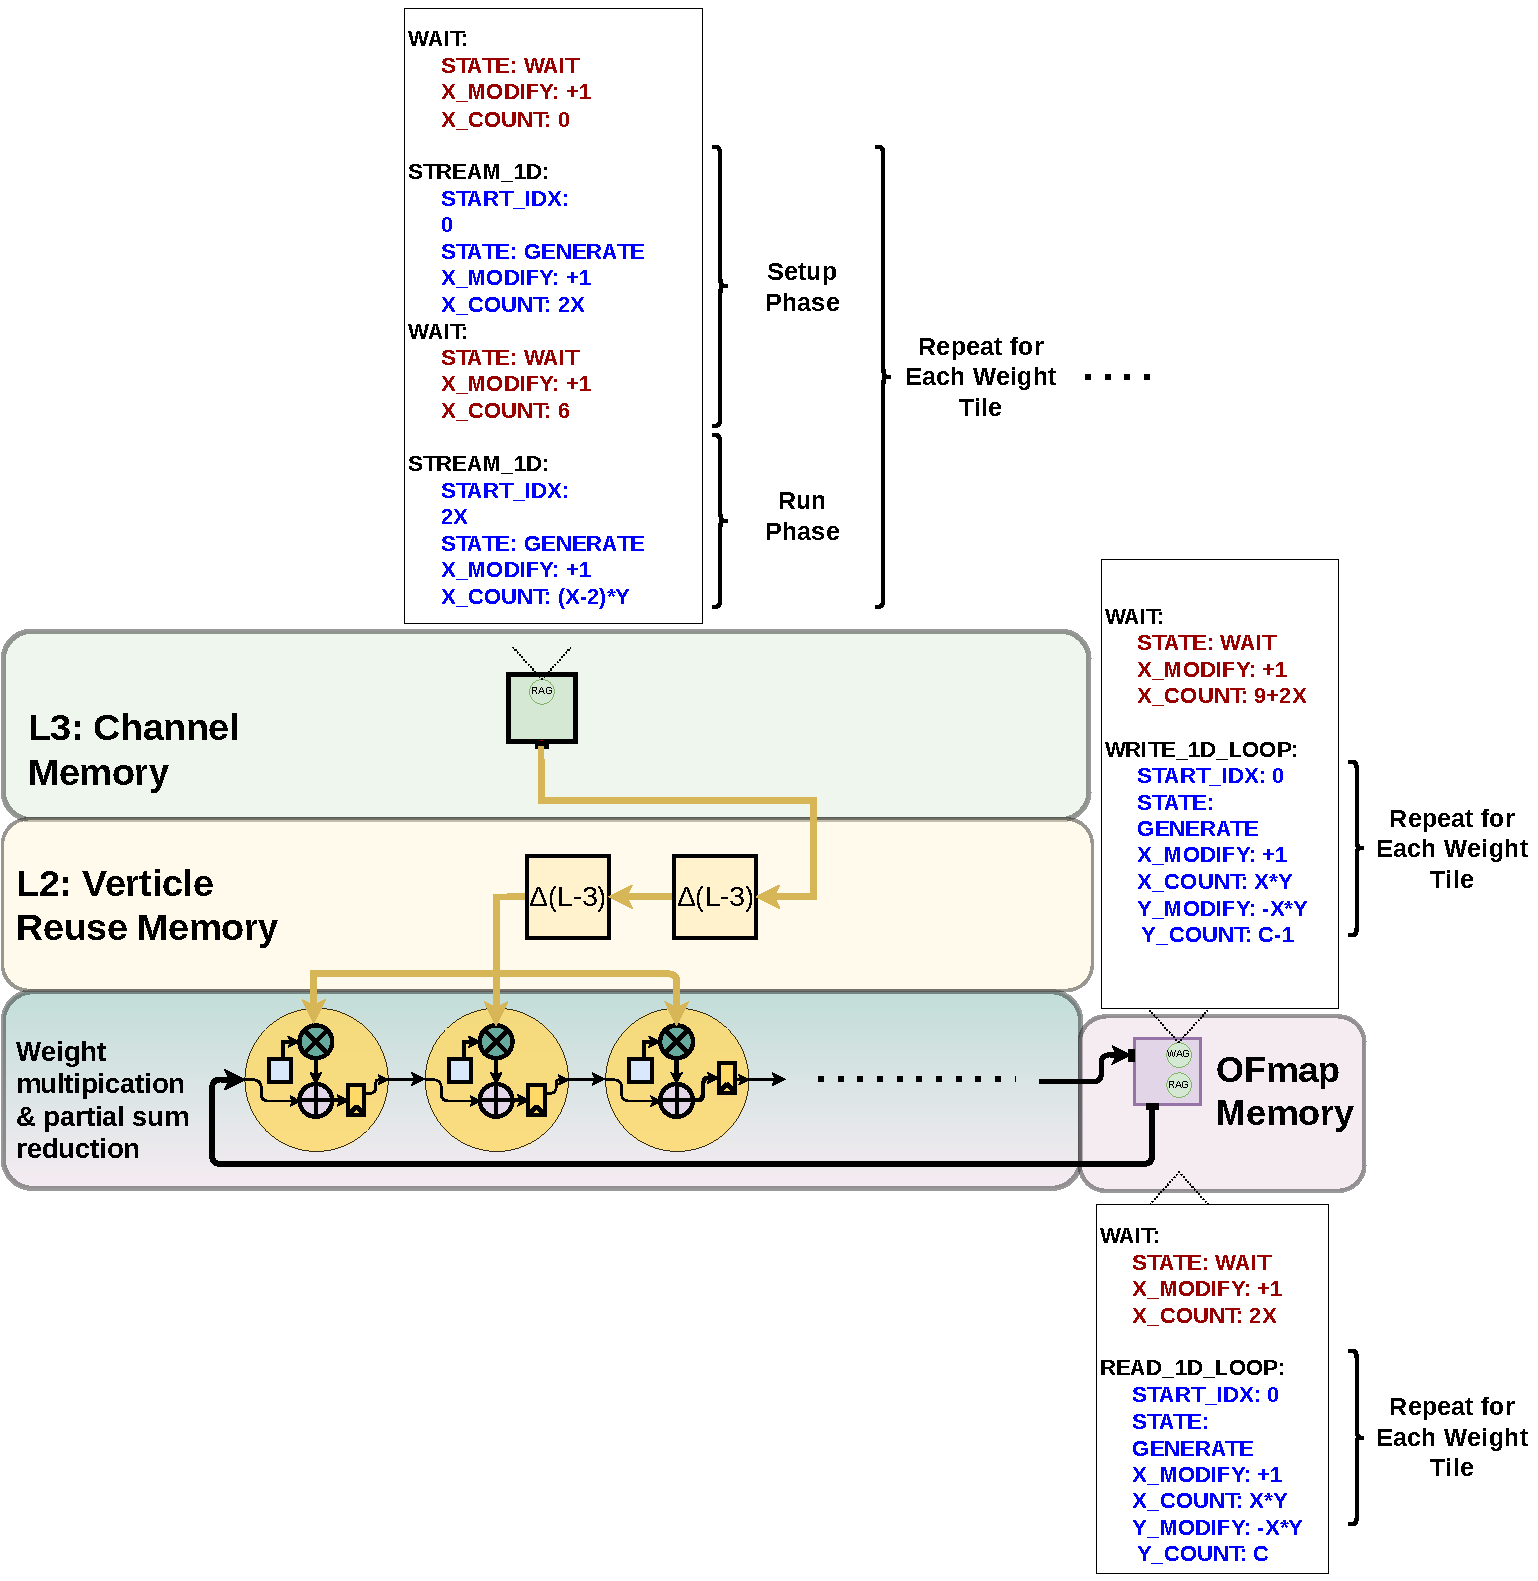
\includegraphics[scale=0.495]{fig/3x3conv_sched.pdf}
    \caption{Illustration of (1, 1) convolution scheduling}
    \label{fig:3x3conv_sched}
\end{figure}